\section{Traditional Computing Platform}

\subsection{Generalized Distributed Resource Management System Architecture}

Dynamic Distributed Resource Management Systems usually have a centralized
control and thus can be split into two layers, the control plane and the data
plane.

\begin{figure}[h!]
  \centering
  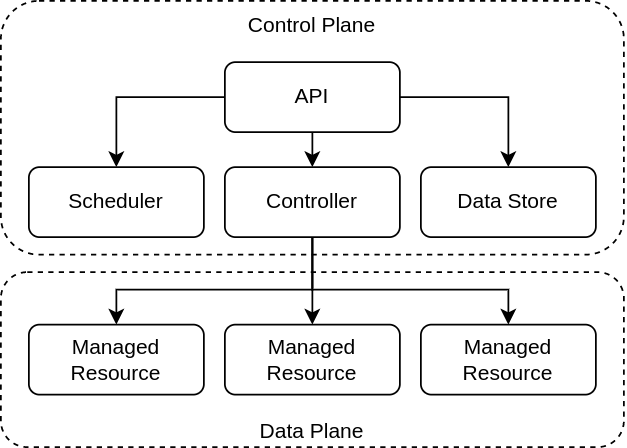
\includegraphics[width=0.6\linewidth]{resources/dynamic-distributed-resource-management-overview.png}
  \caption{Overview over general components in a Dynamic Distributed Resource Management System}
  \label{fig:ddrms-overview}
\end{figure}

The control plane is a set of components that make global decisions about the
distributed system as a whole and acts as a single source of truth regarding the
configuration and state of all components and resources in the distributed
system.

The control plane generally consists of the following components:

\begin{description}
  \item[Data Store]
    Responsible for consistently storing the current configuration and state of
    all components and resources.
  \item[API]
    An interface for users, administrators, and other components in the
    distributed system to interact with.
  \item[Controller(s)]
    A component or set of components responsible for managing all or a specific
    type of computing resources.
  \item[Scheduler]
    Component responsible with determining the physical or virtual location of a
    newly requested computing resource.
\end{description}

The data plane aggregates the computing resources managed by the control plane,
for instance virtual or physical machines, storage, networks, or more abstract
resources like services, tasks, or secrets.

Customers usually interact with the system by using for example graphical or
terminal applications. There are no additional services that are expected to be
managed by the customer.

\subsection{Services Models}

\citetitle{mell2011} \cite{mell2011} defines three distinct models.

\subsubsection{Infrastructure as a Service (IaaS)}

In an IaaS service model the managed resources are classical computing
resources. This includes -- physical or virtual -- machines, storage, and
networks.

\subsubsection{Platform as a Service (PaaS)}

A computing platform is an environment in which an application is executed.
The infrastructure the execution environments are created on is either also
managed by the platform or is provided by an infrastructure service provider.

Service providers offering a PaaS service model usually not only provide the
execution environment for an application but also offer services like
aggregation of logs and metrics and monitoring said applications. The data
needed for these additional services is provided by the control plane.

To summarize the responsibilities and needed privileges the control plane has on
the platform:

\begin{itemize}
  \item Creating execution environments on provided infrastructure
  \item Executing applications in said execution environment
  \item Monitoring those applications
  \item Aggregating metrics and logs
\end{itemize}

In this architecture could execute arbitrary applications in an execution
environment provided to a customer, making it impossible to shield data inside
said execution environment. Application logs could also contain sensitive data,
which are fully accessible by the platform control plane.


